%	PACKAGES AND OTHER DOCUMENT CONFIGURATIONS

\documentclass[11pt, a4paper,twocolumn]{article} % 10pt font size (11 and 12 also possible), A4 paper (letterpaper for US letter) and two column layout (remove for one column) Use additional titlepage argument to generate this
%\documentclass[12pt, a4paper,twocolumn,titlepage]{article}

\input{structure.tex} % Specifies the document structure and loads requires packages
\graphicspath{{"/Users/Kit/OneDrive/Documents/Computing/Trojan Asteroids/Report/Figures"}}


%	ARTICLE INFORMATION

\title{Modelling the Trojan Asteroids}
%\subtitle{Blue Organic Light Emitting Diodes using Thermally Activated Delayed Fluorescence}

%\author{
	%\authorstyle{Christopher Gallagher}}
\author{\authorstyle{Christopher Gallagher} 
	\institution{University of Cambridge}}
% Example of a one line author/institution relationship
%\author{\newauthor{John Marston} \newinstitution{Universidad Nacional Autónoma de México, Mexico City, Mexico}}

\date{\today} % Add a date here if you would like one to appear underneath the title block, use \today for the current date, leave empty for no date
\usepackage[english]{babel}
\usepackage{tabularx}
%\usepackage[backend=biber,doi=false]{biblatex}
\addbibresource{references.bib}
%\AtBeginBibliography{\small}
%----------------------------------------------------------------------------------------
\begin{document}

\maketitle % Print the title

\thispagestyle{firstpage} % Apply the page style for the first page (no headers and footers)

%	ABSTRACT

\lettrineabstract{Trojan asteroids are v important. I'm going to make that paragraph a little longer to fill out the space in case this is forming some kind of error. i really hope this is long enough.}

%	ARTICLE CONTENTS

%Use https://leancrew.com/all-this/2016/08/lagrange-points-redux/ to create your own contour plot?
\section{Introduction}
The Jupiter trojans, commonly known as the Trojan asteroids, are two large groups of asteroids that share the planet Jupiter's orbit around the Sun in a 1:1 orbit resonance. These two groups are called the Greeks and the Trojans, named after opposing sides in the mythological Trojan war, and lead/trail Jupiter respectively in its orbit. They correspond to Jupiter's two stable Lagrange points: L\subscript{4}, lying 60° ahead of the planet in its orbit, and L\subscript{5}, 60° behind, with asteroids distributed in two elongated, curved regions around these Lagrangian points. 

The first Jupiter trojan, 588 Achilles, was discovered in 1906 by the German astronomer Max Wolf \cite{Nicholson1961}, and a total of 7642 Jupiter trojans have been found as of February 2020 \cite{IAU2020}.

Research into Jupiter's trojan asteroids continues, with the particular focus on their origins reliant on an understanding of their orbit stability \cite{DiSisto2019}, \cite{Nesvorn2018}. This informs studies into their composition \cite{Brown2016}, as travel to these asteroids is considered for their potential in mineral mining \cite{Okada2017} \cite{Levison2016}. 

The purpose of this report is to use numerical simulation techniques to investigate the stability of orbits about these Lagrange points, demonstrating the asteroid oscillate about these points under small perturbations and quantifying the absolute distance of the asteroids from the Lagrange point (the wander) during their orbits. The impact of variation in planetary/solar mass on asteroid orbit stability will also be considered. \textit{Signpost what is included in each section?}

% \cite{Nakamura2008} gives spatial distribution

\section{Theoretical Background?}

\subsection{Lagrange Points}
The asteroids exist at/near Lagrange points, defined in Lagrange's initial analysis of the three-body problem in 1772 \cite{Lagrange1772}, were he demonstrated the existence of five equilibrium points for an object of negligible mass orbiting under the gravitational effect of two larger masses. Three of these equilibrium points, L\subscript{1}-L\subscript{3} lie on the line joining the two masses, while each of the remaining two points, L\subscript{4} and L\subscript{5}, lie at the apex of an equilateral triangle with base equal to the separation of the two masses (see Figure \ref{fig:lagrangepoints}). Despite all these points being potential maxima, stable motion is possible around L\subscript{4} and L\subscript{5} due to the Coriolis force \cite{Lissauer2014}.
%lissauer also says stability is provided that the most massive body has at least 25 times the mass of the secondary

\begin{figure}[h]
	\centering
	\includegraphics[width=\linewidth]{Figures/lagrange_points}
	\caption{The location of the five Lagrange equilibrium points in the circular-restricted three-body problem. The solar and planetary masses are denoted by the large and small filled circles, and the letters P, H, and T denote passing, horseshoe, and tadpole orbits respectively. Note that the two masses form an equilateral triangle with each of the L\subscript{4} and L\subscript{5} points. Reproduced from Marzari et al. \cite{Marzari2002}}
	\label{fig:lagrangepoints}
\end{figure}

While orbits between Lagrange points are also possible, this report will focus on the tadpole orbits observed as asteroids deviate from L4 and L5 \cite{Murray1999}. \textit{More detail?}


\subsection{Theoretical Model}
The three body problem, where the dynamics of three interacting bodies are determined given their initial positions and velocities, has no analytical (closed-form) solution in the general case \cite{Barrow2008}.

In this report, I will consider the circular, restricted, three-body problem, where two of the bodies move in circular, coplanar orbits about their common centre of mass, unaffected by the negligible mass of the third body. I will also assume that all interactions are via Newtonian gravity.

The system of differential coordinates determine the position and velocity of the asteroids, with two equations per spatial coordinate.
\begin{equation}
\frac{dr_{i}}{dt} = v_{i}, \frac{dv_{i}}{dt} = g_{i}, \quad i = x,y 
\end{equation}

In this, $g_{i}$ is given by:
\begin{equation}
\textbf{g}= - \frac{G M_{s}}{\lvert \textbf{r} - \textbf{r}_{s} \rvert ^{3}} (\textbf{r} - \textbf{r}_{s})
		 - \frac{G M_{p}}{\lvert \textbf{r} - \textbf{r}_{p} \rvert ^{3}} (\textbf{r} - \textbf{r}_{p})
\end{equation}
where the subscripts \textit{s} and \textit{p} refer to solar and planetary properties respectively.

We may also consider a frame rotating at the same speed as the massive bodies. As there is 1:1 orbital resonance between Jupiter and the asteroids, all three bodies are stationary in this frame. This significantly increases the accuracy of numerical simulations, as \textbf{WHY}

When transforming into this rotating non-inertial frame, $g_{i}$ gains an additional virtual force term with coupling between the spatial coordinates. This is given below as the sum of the centripetal and Coriolis forces:

\begin{equation}
\Delta g_{i} = \Omega^{2} r_{i} - 2[\bm{\Omega} \times \textbf{v}]_{i}
\end{equation}
where $\Omega$ is the angular speed of the rotating frame, and $\textbf{v}$ is the velocity of the asteroid within this frame. 


\subsubsection{Assumptions - FIX}
\begin{itemize}
	\item Circular orbit
	\item Constant Jupiter-Sun separation
	\item Coplanar orbits
	\item Negligible asteroid mass
	\item Newtonian gravity
\end{itemize}

I also applied the following symmetries:
trojan and greek symmetry (analysis focused on greeks)
rotational symmetry - arbitrary initial point 
direction of orbit
"The combination of these symmetries allows the problem to be simplified. Such that
only the Greeks, orbiting counter-clockwise, with perturbations at t = 0, need to be
investigated.
"
(This reduces computing time not hvaing to solve for trojans as well)

\subsection{Orbit Geometry}
As the three bodies considered here form an equilateral triangle in the initial equilibrium state, as depicted in Figure \ref{fig:geometry}, we can derive the polar coordinates of each body with respect to the centre of mass about which the bodies orbit.

\begin{figure}
	\centering
	\resizebox{\columnwidth}{!}{%
		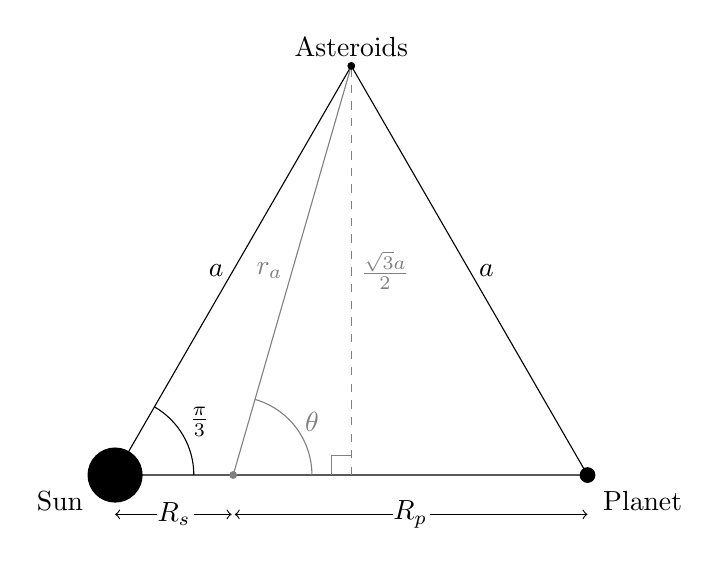
\begin{tikzpicture}
		\draw (0,0) -- (6,0) -- (3, {6*sin(60)} ) node[above]{Asteroids} node[midway,right]{$a$} -- cycle node[midway,left]{$a$};
		\draw  (1,0) arc (0:60:1cm)  ;
		%\node [label={[shift = {(10mm,5mm)}]{$\frac{\pi}{3}$}}] {};
		\node [label={[shift = {(13:11mm)}]{$\frac{\pi}{3}$}}] {};
		\node [label={[shift = {(-7mm,-7mm)}]{Sun}}] {};
		\node [label={[shift = {(67mm,-7mm)}]{Planet}}] {};
		
		\fill[gray] ({6*(1/4)}, 0) circle (0.5mm);
		\draw[gray] ({6*(1/4)}, 0) -- (3, {6*sin(60)} ) node[midway,left]{$r_{a}$};
		\draw[dashed, gray] (3, 0) -- (3, {6*sin(60)} )node[midway,right]{$\frac{\sqrt{3}a}{2}$};
		\draw[gray]  ({6*(1/4) + 1}, 0) arc (0:{atan(4*sin(60))}:1cm)  ;
		\node [label={[gray, shift = {(25mm,3mm)}]$\theta$}] {};
		\draw[gray] (2.75,0) -- (2.75, 0.25) -- (3, 0.25);
		
		\draw[arrows=<-](0,-0.5)--(0.53,-0.5);
		\node at (0.75, -0.5) {$R_s$};
		\draw[arrows=->](1.0,-0.5)--(1.48,-0.5);
		
		\draw[arrows=<-](1.52,-0.5)--(3.53,-0.5);
		\node at (3.75, -0.5) {$R_p$};
		\draw[arrows=->](4.00,-0.5)--(6,-0.5);
		
		%\draw[arrows=<-](0,-1)--(2.88,-1);
		%\node at (3, -1) {$a$};
		%\draw[arrows=->](3.1,-1)--(6, -1);
		
		\fill[black] (0,0) circle (3.5mm);% node[anchor=north west] {Sun};
		\fill[black] (6,0) circle (1mm);
		\fill[black] (3, {6*sin(60)} ) circle (0.5mm);
		
		\end{tikzpicture}
	}	
	\caption{A geometric depiction of the three-body system, in the case where the planet has a mass equal to a third of the sun, and asteroids are considered at the L\subscript{4} point. $ R_{s} $ and $ R_{p}$ denote the (fixed) radii from the centre of mass (the grey point) to the Sun and the planet respectively, while $ r_{a} $ denotes the radius of the asteroids.}
	\label{fig:geometry}
\end{figure}

Using standard trigonometric relations, it is simple to show that the values $ r_{a} $ and $ \theta $ are given by:

\begin{equation}
r_{a} = \sqrt{a^{2} + R_{s} R_{p}} , \enspace \theta =  \tan^{-1} \left( \frac{a \sin(\frac{\pi}{3})}{R_{p} - \frac{a}{2}} \right)
\end{equation}

Furthermore, the Lagrange point in Cartesian coordinates based about the centre of mass is easily found to be:

\begin{equation}
(x,y) = \left( R_{p} - \frac{a}{2}, \frac{ \sqrt{3} a}{2} \right)
\end{equation}

Finally, equating the gravitational and centripetal forces on the planet allows the derivation of its (and all other bodies') orbital velocity:

\begin{equation}
\Omega = \sqrt{\frac{G (M_{s} + M_{p})}{a^{3}}}
\end{equation}

\section{Methodology}
This system of coupled first-order differential equations was solved using the scipy solve\_ivp function. The time span was taken as 100 orbits (with 100 points sampled per orbit) unless otherwise stated; this corresponds to 1185 Earth years. Rescaled solar system units are used for mathematical ease, so distances are measured in astronomical units (AU), time in earth years and mass in multiples of the solar mass, and to prevent floating point overflows due to the magnitude of the quantities considered in SI units.


The wander was defined as the maximum distance of the asteroid from the initial point during the orbit (for small perturbations this is also approximately the separation from the Lagrange point).
Initial conditions are defined by the Lagrange point in each frame, with the initial velocity in the stationary frame defined by the period of Jupiter's orbit, and split into Cartesian components.

\subsection{Integration Method}
%Put this with theory as "numerical methods"?
%Then all theory could be in methodology?
Within solve\_ivp, the default solver is RK45 (an explicit Runge-Kutta method of order 5(4) \cite{Dormand1980}) however this is non-stiff, giving a deviation in asteroid position (from the Lagrange point) in the order of $ 10^{-4}$ AU in the rotating frame over 50 years. This is larger than expected, suggesting the system of equations requires an unreasonable small step size for  numerically stability with respect to this numerical method, even regions where the solution curve is smooth \cite{Lambert1991}. This suggests the system is stiff, and solvers designed for this typically do more work per step, allowing them to take much larger steps, and have improved numerical stability compared to the non-stiff solvers \cite{Byrne1987}. 

Instead the stiff "Radau" solver (an implicit Runge-Kutta method of the Radau IIA family of order 5 \cite{Hairer2010}) is used for increased stability \cite{Frank1985}, and achieves a deviation in asteroid position in the order of $ 10^{-13}$ AU instead. This also ensures stability in the rotating frame, with deviations of 0.76\% in asteroid separation from Jupiter over $ 10^{3} $ years, compared to 53\% for the best non-stiff solvers.

%Can add more detail on A vs B stability (I believe B stability is relevant here but maybe check this)

\subsection{Programme Structure}
Global constants such as solar mass, and sun\textendash planet separation, along with derived values from these such as orbital period and solar radius from centre of mass, as given in an importable python module "\textit{constants}".

Functions to evaluate these coupled differential equation systems are defined in module "\textit{orbits}", while additional functions to evaluate the wander during the orbit (under different sampling routines) are implemented in "\textit{wander}". Further files then import these modules and produce the plots given in this report.

To consider a varying planet mass, it was considered preferable to avoid reconstructing all functions to take this as an argument as this requires re-evaluating all initial derived constants. Therefore, I iterate over alternative masses, re-defining constant values in this instance, and then directly import the required functions to compute the orbit. \textbf{REPHRASE?}

Complete code listings are given in appendix \ref{Code}.


\section{Results}
\subsection{Orbit Stability}
\subsection{Wander Analysis}
\subsubsection{Perturbations in z-direction}

\section{Discussion}
\section{Conclusion}



%Talk about animations here too? or after solver method
\printbibliography

\onecolumn
\begin{appendices}

\section{Code 1} \label{Code}
\begin{lstlisting}[language=Python]
import math
import numpy as np
from scipy import integrate
import matplotlib.pyplot as plt

from constants import G, M_S, M_P, R, ORBIT_NUM, PRECISION  # User defined constants
from constants import (
	solar_rad,
	planet_rad,
	period,
	omega,
	time_span,
)  # Derived constants


\end{lstlisting}
%Can add my own style guide to this, see suggestions on https://www.overleaf.com/learn/latex/code_listing
%\section{Code 2}

\end{appendices}

\end{document}

%%%%%%%%%%%%%%%%%%%%%%%%%%%%%%%%%%%%%%%%%
% Wenneker Article
% LaTeX Template
% Version 2.0 (28/2/17)
%
% This template was downloaded from:
% http://www.LaTeXTemplates.com
%
% Authors:
% Vel (vel@LaTeXTemplates.com)
% Frits Wenneker
%
% License:
% CC BY-NC-SA 3.0 (http://creativecommons.org/licenses/by-nc-sa/3.0/)
%
%%%%%%%%%%%%%%%%%%%%%%%%%%%%%%%%%%%%%%%%%
